%%%%%%%%%%%%%%%%%%%%%%%%%%%%%%%%%%%%%%%%%%%%%%%%%%%%%%%%%%%%%%%%%%%%
%% I, the copyright holder of this work, release this work into the
%% public domain. This applies worldwide. In some countries this may
%% not be legally possible; if so: I grant anyone the right to use
%% this work for any purpose, without any conditions, unless such
%% conditions are required by law.
%%%%%%%%%%%%%%%%%%%%%%%%%%%%%%%%%%%%%%%%%%%%%%%%%%%%%%%%%%%%%%%%%%%%
\PassOptionsToPackage{svgnames}{xcolor}

\documentclass[
  digital, %% This option enables the default options for the
           %% digital version of a document. Replace with `printed`
           %% to enable the default options for the printed version
           %% of a document.
  oneside, %% This option enables double-sided typesetting. Use at
           %% least 120 g/m² paper to prevent show-through. Replace
           %% with `oneside` to use one-sided typesetting; use only
           %% if you don’t have access to a double-sided printer,
           %% or if one-sided typesetting is a formal requirement
           %% at your faculty.
  table,   %% This option causes the coloring of tables. Replace
           %% with `notable` to restore plain LaTeX tables.
  nolof,     %% This option prints the List of Figures. Replace with
           %% `nolof` to hide the List of Figures.
  nolot,     %% This option prints the List of Tables. Replace with
           %% `nolot` to hide the List of Tables.
  %% More options are listed in the user guide at
  %% <http://mirrors.ctan.org/macros/latex/contrib/fithesis/guide/mu/fi.pdf>.
]{fithesis3}
%% The following section sets up the locales used in the thesis.
\usepackage[resetfonts]{cmap} %% We need to load the T2A font encoding
\usepackage[T1,T2A]{fontenc}  %% to use the Cyrillic fonts with Russian texts.
\usepackage[
  main=english, %% By using `czech` or `slovak` as the main locale
                %% instead of `english`, you can typeset the thesis
                %% in either Czech or Slovak, respectively.
  english, german, russian, czech, slovak %% The additional keys allow
]{babel}        %% foreign texts to be typeset as follows:
%%
%%   \begin{otherlanguage}{german}  ... \end{otherlanguage}
%%   \begin{otherlanguage}{russian} ... \end{otherlanguage}
%%   \begin{otherlanguage}{czech}   ... \end{otherlanguage}
%%   \begin{otherlanguage}{slovak}  ... \end{otherlanguage}
%%
%% For non-Latin scripts, it may be necessary to load additional
%% fonts:
\usepackage{paratype}
\def\textrussian#1{{\usefont{T2A}{PTSerif-TLF}{m}{rm}#1}}
%%
%% The following section sets up the metadata of the thesis.
\thesissetup{
    date          = \the\year/\the\month/\the\day,
    university    = mu,
    faculty       = fi,
    type          = mgr,
    author        = Bc. Andrej Staruch,
    gender        = m,
    advisor       = {RNDr. Marek Kumpošt, Ph.D.},
    title         = {Aplikace pro detekci phishing útoků na základě testování URL},
    TeXtitle      = {Aplikace pro detekci phishing útoků na základě testování URL},
    keywords      = {phishing detection, Phishtank, security, cpp, 
javascript, URL tests, Trusted Network Solutions},
    TeXkeywords   = {phishing detection, Phishtank, security, cpp, 
javascript, URL tests, Trusted Network Solutions},
    abstract      = {The goal of this master's thesis is to design and implement a system, which will compute potential risk for a given URL. The computation of potential risk is based on extendable series of individual test suites, and the result of weighted tests is a number called 'phishing score'. Based on this number, the application can automatically allow or block the given communication. Optionally, the end user could be warned and decide if he wants to proceed to this website.
    },
    % thanks        = {These are the acknowledgements for my thesis, Mgr. Karol Kubanda, učo 143339 (konzultant) },
    bib           = example.bib,
}
% http://blog.chapagain.com.np/latex-numbering-subsubsection-and-showing-it-in-table-of-contents/


\usepackage{makeidx}      %% The `makeidx` package contains
\makeindex                %% helper commands for index typesetting.
%% These additional packages are used within the document:
\usepackage{paralist} %% Compact list environments
\usepackage{amsmath}  %% Mathematics
\usepackage{amsthm}
\usepackage{amsfonts}
\usepackage{url}      %% Hyperlinks
\PassOptionsToPackage{hyphens}{url}\usepackage{hyperref}
\usepackage{markdown} %% Lightweight markup
\usepackage{listings} %% Source code highlighting
\usepackage{booktabs}
\usepackage{tabularx}
\usepackage{dirtree}
\usepackage{csquotes}
\usepackage{pgfplots} % barplot graph
\usepgfplotslibrary{dateplot}
\pgfplotsset{compat=1.12}

% https://tex.stackexchange.com/questions/120336/adding-several-labels-year-month-to-a-graph-in-pgfplots
\makeatletter
\long\def\ifnodedefined#1#2#3{%
    \@ifundefined{pgf@sh@ns@#1}{#3}{#2}%
}
\makeatother

%% https://tex.stackexchange.com/questions/2504/beamer-blocks-in-ordinary-article-style-document
\usepackage{tcolorbox}
\usepackage{lipsum}
\tcbuselibrary{skins,breakable}
\usetikzlibrary{shadings,shadows}

% Numbering also for subsubsection
% fithesis/style/mu/fithesis-base.sty:498:\setcounter{secnumdepth}{3}
% \setcounter{secnumdepth}{3} <- this is overrided in fithesis-base


\newenvironment{myexampleblock}[1]{%
    \tcolorbox[beamer,%
    noparskip,breakable,
    colback=LightGreen,colframe=DarkGreen,%
    colbacklower=LimeGreen!75!LightGreen,%
    title=#1]}%
    {\endtcolorbox}

\newenvironment{myalertblock}[1]{%
    \tcolorbox[beamer,%
    noparskip,breakable,
    colback=LightCoral,colframe=DarkRed,%
    colbacklower=Tomato!75!LightCoral,%
    title=#1]}%
    {\endtcolorbox}

\newenvironment{myblock}[1]{%
    \tcolorbox[beamer,%
    noparskip,breakable,
    colback=LightBlue,colframe=DarkBlue,%
    colbacklower=DarkBlue!75!LightBlue,%
    title=#1]}%
    {\endtcolorbox}
    
\newcounter{feature}
\newenvironment{feature}[1]{\stepcounter{feature}%
    \tcolorbox[beamer,%
    noparskip,breakable,
    colback=LightBlue,colframe=DarkBlue,%
    colbacklower=DarkBlue!75!LightBlue,%
    title=Feature~\thefeature: #1]}%
    {\endtcolorbox}
    



\lstset{
  basicstyle      = \ttfamily,%
  identifierstyle = \color{black},%
  keywordstyle    = \color{blue},%
  keywordstyle    = {[2]\color{cyan}},%
  keywordstyle    = {[3]\color{olive}},%
  stringstyle     = \color{teal},%
  commentstyle    = \itshape\color{magenta}}
\usepackage{floatrow} %% Putting captions above tables
\floatsetup[table]{capposition=top}

%%% author on next line
%%% https://tex.stackexchange.com/questions/351733/csquotes-and-beamer-citation-for-blockquote-flush-right-on-separate-line?noredirect=1
\renewcommand{\mkblockquote}[4]{#1#2\newline\null\hfill\rule{0.5\textwidth}{0.1pt}\newline\null\hfill\footnotesize{#4#3}}

    
\begin{document}
\chapter{Introduction}

\nocite{apwg-2012-4}
\nocite{apwg-2013-1}
\nocite{apwg-2013-2}
\nocite{apwg-2013-3}
\nocite{apwg-2013-4}
\nocite{apwg-2014-1}
\nocite{apwg-2014-2}
\nocite{apwg-2014-3}
\nocite{apwg-2014-4}
\nocite{apwg-2015-1}
\nocite{apwg-2015-4}
\nocite{apwg-2016-1}
\nocite{apwg-2016-2}
\nocite{apwg-2016-3}
\nocite{apwg-2016-4}
\nocite{apwg-2017-1}
\nocite{apwg-2017-3}
\nocite{apwg-2017-4}
\nocite{apwg-2018-1}
\nocite{apwg-2018-2}
\nocite{apwg-2018-3}
\nocite{apwg-2018-4}
\nocite{apwg-2019-1}
\nocite{apwg-2019-2}

In today's world, the threat of a cyber attack can't be ignored. There are a plethora of companies that try to protect their customers from potential damage, such as getting infected by a virus, getting ransomware or malware or protect their business intelligence.

This thesis is concerned with another part of the cyber crime called phishing. Phishing is a social engineering attack to obtain sensitive information such as user names, passwords, credit card details, bank account credentials for malicious reasons.  Because of a large attack vector, there isn't a reliable way or a tool to prevent such an attack consistently in every sector.

This thesis will review several ways to detect a phishing attack, implement some of them and test them in the production environment with an association with a Trusted Network Solutions company. The final software could be easily used with another proxy or tool.

First of all, we'll look around current market for existing solutions for phishing protection and compare them. After that, we will look for academic papers with phishing oriented thematic and review different approaches and choose suitable ones. Following these steps, we will design and implement phishing detection system. After that, we will test it on real customer traffic and conclude to result whether security of users has increased or not.

Designing an anti-phishing system has similar character as designing an anti-virus system - we are trying to protect user before malicious attempts of an attacker but as we can see, users are still infected when they are using anti-virus, so designing correct and powerful anti-phishing system is an uneasy task. We will focus on extendability for future editions.

% The word phishing is originated from the word fishing - attackers fishes on their victims. Phishers use a number of techniques to trick their possible victims: having a fake clone site like the original one with forms so a user will enter credentials to their site, or sending e-mails with messages to send money to some address.


% TODO: cite the organization APWG
% Nezisková organizácia APWG, ktorá ma za cieľ zjednotiť obranu voči cyberútokom, pravidelne vytvára štatistiky o aktuálnych trendoch a počtoch phishing útokov. Na číslach za uplynulý pol rok je vidno, že sa celkový počet pohybuje v podobnej rovine:

% Počet jednotlivých stránok má rôzne výkyvy, zatiaľ čo počet e-mailov sa postupne zvyšuje. Na základe analýz životnosti jednotlivých phishingových kampaní sa zistilo, že priemerná živostnosť je okolo 12 hodín [2]. Táto skutočnosť výrazne ovplyvňuje schopnosť automaticky detekovať phishingový útok (doplniť rozumný dôvod, citáciu).

% TODO: spomenúť význam tejto práce, že sa ešte nenachádza komplexné riešenie pre integráciu do proxy pre lokálny trh

% TODO: poriadne odcitovať všetky horné poznatky aby to nebol kompilát.

% TODO: Pridať odstavec o detekcii na základe vizuálnej podobnosti.

% TODO: pridať odstavec ohľadom toho, že táto práca bude slúžiť ako ochrana pre užívateľov za proxy.

\chapter{Theoretical background}

What is a phishing? Many academic papers or security companies have different definition for phishing. We can look at them to have a broader look for this problem, thus every one add its own bit:

\blockquote[Certain Investigation on Web Application Security \cite{certain-investigation}][]{
Phishing    is    a    trap    where    any    targeted    individual,    is    communicated  by  someone  impersonating  as  a  legitimate  and  a  reputed  organization  to  entice  the  individual  into  providing  sensitive information such as banking information, credit card details, and  passwords.
}

\par

\blockquote[Phishing Detection: A Literature Survey \cite{literature-survey}][]{
\par Phishing is a social engineering attack that aims at exploiting the weakness found in system processes as caused by system users.
}


\blockquote[A secured methodology for anti-phishing \cite{secured-methodology}][]{
\par The   technique   used   to   perform   on-line   robbery/stealing  of  person  credentials  is  called  phishing  in cyber international.
}

\par

In short words, its fraudulent attempt combining social engineering skills with a technical trickery to obtain sensitive data from other parties. 

For a more exhaustive definition, we can peek at Anti-Phishing World Group definition, that covers most of the previous definitions:

\blockquote[Phishing Activity Trends Report \cite{apwg-2019-2}][]{
Phishing is a criminal mechanism employing both social
engineering and technical subterfuge to steal consumers’
personal identity data and financial account credentials.
Social engineering schemes use spoofed e-mails
purporting to be from legitimate businesses and
agencies, designed to lead consumers to counterfeit Web
sites that trick recipients into divulging financial data
such as usernames and passwords. Technical subterfuge
schemes plant crimeware \footnote{\url{https://en.wikipedia.org/wiki/Crimeware}} onto computers to steal
credentials directly, often using systems to intercept
consumers’ account user names and passwords -- and to
corrupt local navigational infrastructures to misdirect
consumers to counterfeit Web sites (or authentic Web
sites through phisher-controlled proxies used to monitor
and intercept consumers’ keystrokes).
}









\section{Phishing strategies}

Phishing attacks are usually divided into several categories based on the who is the target:
\begin{enumerate}
    \item Deceptive phishing - this is the most common attack where an attacker is trying to steal money from the victim, usually done by sending a fake email from a bank with a fake URL link, where account details are exposed to the attacker. This attack is typically done in batches on large group of victims, typically some leaked database with e-mails.
    \item Spear phishing - this attack involves more social engineering skills and is targeted on single units instead of a wide group like in deceptive phishing. Attackers need to perform detailed research of their victim making it difficult to mark this attack as fraudulent.
    \item Whaling - similar to spear phishing, but attackers take a considerable time to prepare the attack and usually targets executive officers because they have more privileges and knowledge than a common employer.
\end{enumerate}

All of this attacks have in common that the user need to  cooperate with an attacker - open an e-mail, click on the URL, fill the login information on the website.

If user is already on fake site while he believes it's a correct one, it's usually late for him and an attacker gets his credentials. The defence system should prevent him from visiting such site. 

To this date, there has been numerous papers and research about phishing and how to prevent it. We will look thoroughly on them and choose which could fit into our system.

\section{Current defence mechanisms}

\subsection{Browser}

As most of the action \cite{citacia dacoho} from users comes in web browser, the most protection need to be done there. The current software supports some level of protection. For example, Google provides a Google Safe Browsing API (more in section \ref{section:google-safe-browsing} on page \pageref{section:google-safe-browsing}). Then when a user tries to visit deceptive website, there is a built-in defence mechanism preventing a visit the deceptive site (figure \ref{fig:browse-detection}).

TODO: add screenshots from Chrome/Edge/Firefox/Safari Android/iOS

\begin{figure}[h!]
  \caption{Browser detection}
  \centering
  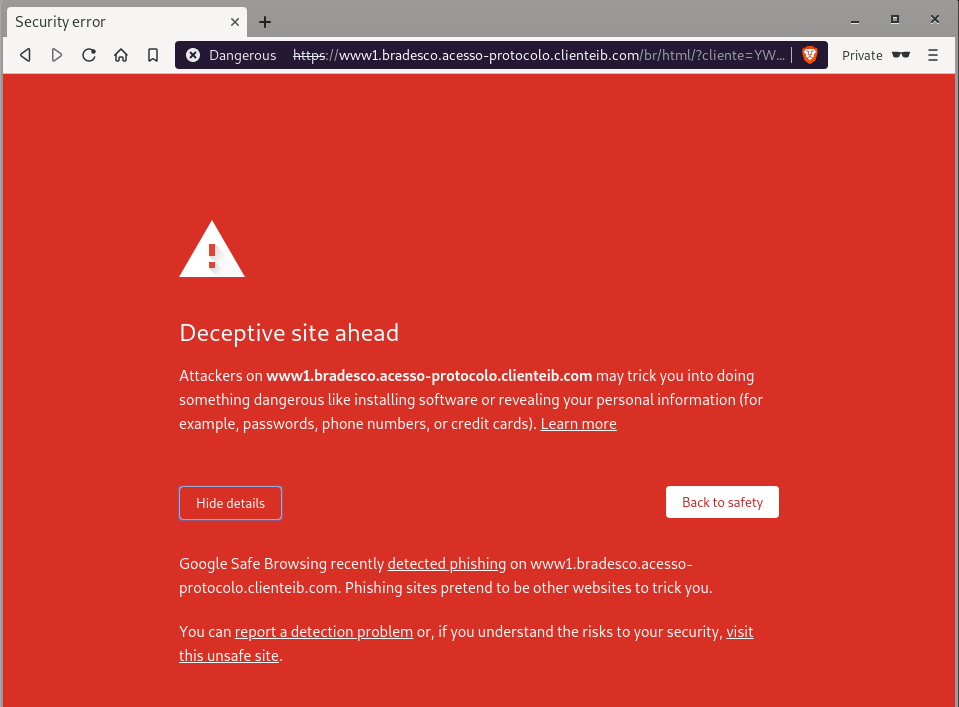
\includegraphics[width=1\textwidth]{images/browser_phishing_detected.png}
  \label{fig:browse-detection}
\end{figure}

\subsection{Anti-virus}



The majority of popular anti-virus technologies also provides some sort of defence mechanism. We will test several of them to compare it to our system in later stage of development. For the whole picture, there is current list of antivirus solutions:
\begin{itemize}
    \item ESET - \href{https://www.eset.com/us/anti-phishing/}{ESET}
    \item AVAST - \href{https://blog.avast.com/avast-improves-phishing-detection-avast}{Avast}
    \item Kaspersky
    \item Norton
    \item Bitdefender
\end{itemize}


\subsection{User education}

If the automatic detection mechanism fail, there is a space for a human factor. The user should be educated, how to look for a signs of phishing site. There are several methods how to educate a user such as briefings with security experts, \cite{citacia na edukaciu} pay the professional teams which tries to breach your company by phishing techniques \cite{citacia na edukaciu} \cite{citacia na edukaciu} or by periodically sending the new/emails from security department on a current state of phishing attacks and how to prevent them.

\section{Trends}

How does phishing developed over the years? We can look at the data from the APWG. They are periodically publishing their reports with current trends, number of phishing websites and campaigns.



Graph: \cite{apwg-2012-4} - \cite{apwg-2019-2}

\begin{figure}[]
  \begin{center}
    \rotatebox[origin=c]{90}{\begin{tikzpicture}
        % \begin{axis}[
        %     width=\linewidth,
        %     date coordinates in=x,
        %     xticklabel={\year/\month},
        %     xlabel=Date (year/month),
        %     ylabel=Y Axis,
        %     legend style={at={(0.5,-0.2)},anchor=north}, % Put the legend below the plot
        %     x tick label style={rotate=90,anchor=east}, % Display labels sideways
        %     xtick=data
        %   ]
    \begin{axis}[
width=17cm,
date coordinates in=x,
% xtick=data,
grid style=dashed,
extra x ticks={2012-10-01, 2013-10-01, 2014-10-01, 2015-10-01, 2016-10-01, 2017-10-01, 2018-10-01, 2019-06-01},
extra x tick style={
    yshift=-3.5ex,
    xticklabel=\year,
    xticklabel style={name={}},
    major tick length=0pt
},
xticklabel style={
    anchor=near xticklabel,
    name=\ifnodedefined{start\year} % Have we already started this year?
        {end\year}  % Then this could be the last month
        {start\year}, % Otherwise, start the year
    append after command=
        \pgfextra{\pgfmathtruncatemacro\lastyear{\year-1}}
        \ifnodedefined{end\lastyear}
        {
                {\ifnum\month=1 (start\lastyear.south west) edge (end\lastyear.south east) \pgfextra{\xdef\finalyear{\year}}\fi}}
        {}
},
after end axis/.code={
    \draw (start\finalyear.south west) -- (end\finalyear.south east);
},
xticklabel=\month,
date ZERO=2012-09-01,% <- improves precision!
]        
            
            
            % add a plot from table; you select the columns by using the actual name in
            % the .csv file (on top)
            \addplot
            table[x=Date,y=E-mail campaigns,col sep=comma] {csv/apwg-stats-email-websites.csv}; 
        \end{axis}
    \end{tikzpicture}
    \caption{Unique phishing campaigns through years}
    }
    % rotatebox
  \end{center}
\end{figure}


\section{Terms \& Glossary \& Wordlist}

\begin{itemize}
    \item HTTP / GET / POST 
    \item REST
    \item API
    \item URL
    \item IPv4
    \item IPv6
    \item DNS 
    \item webpage \& HTML
\end{itemize}

\chapter{Detection methods}
% TODO: this chapter will be about specific approaches and test - why I chose them and why are they beneficial for our app

\section{Detection methods}

Deciding whether the site is phishing or not is not trivial problem. There are many researches and papers with proposed systems that this work derives from. They are mentioning the following approaches:

\subsection{List based approach}

This approach is based on known lists, either  we can white-list or blacklisting - URL coming from this site is phishing, because other URLs from this were classified as malicious. 

The advantage of blacklists with phishing URLs is, that we have certain information about an URL - whether it is a phishing site or not. Somebody had to put it on that site and we can believe it.

There exist services which confronts this problem, some of them are:

\subsubsection{Phishtank}

Phishtank \cite{phishtank} is an online collaborative tool to track and share phishing data. Anyone can submit fraudulent URLs, users then verify if a given website is a phishing site or not. Phishtank provides a public API  where a client can perform a lookup for one URL through the POST request \footnote{\href{https://www.phishtank.com/api_info.php}{https://www.phishtank.com/api\_info.php}}, or he can request a current snapshot of the database \footnote{https://www.phishtank.com/developer\_info.php}. 

\subsubsection{OpenPhish}

OpenPhish \cite{openphish} is automated platform for phishing intelligence. It analyses given URLs from various partners, and if an URL is a phishing one, its provides variety of metadata and information. Then the platform provides a list with live phishing URLs. 

\subsubsection{Google Safe Browsing}
\label{section:google-safe-browsing}

Google provides it's own lists through a Safe Browsing API \cite{google-safe-browsing}. The client application can query the API and get information if has any threat type (malware, social engineering or other).

Last two methods are slightly different than previous, because they are working only with hostnames/domains, instead of whole URLs.

\subsubsection{DNSBL}

Domain Name System-based Blackhole List \cite{wiki:dnsbl} is used for real time stopping of the spam. Spam campaings are usually going together \cite{najdi daku citaciu} with phishing campaigns. Lookup in DNSBL is performed through DNS "A" records. If record is returned, than host is blacklisted. If domain is not listed (and thus its clear), NXDOMAIN is returned.

\subsubsection{DNSWL}

DNS-based whitelist \cite{wiki:dnswl} has on a contratry other approach - locations of IP addresses or hosts, which are consistent and have low percentage of a spam. This option is mainly for future extentions, because black listing is not possible for many host in IPv6 universe.

List-based approach also has big disadvantage - it's not reactive enough. As stated in \cite{najdi pojebanu citaciu kde si to cital} an average phishing campaign lasts only about 2 hours. This is usually too short amount of time to send an URL to a service, categorize it manually, and deploy it in blacklist. Because of this, we need to look for another approaches. 

\subsection{URL analysis}

%% An Assessment of Features Related to Phishing Websites using an Automated Technique

Download a Phishtank db and give initial score to the features based on how many of them has this feature.

In the work from 2012 \cite{url-features-work}, they are suggesting the following techniques for analyzing following URL features:

\subsubsection{Usage of the IP address \cite{url-features-work} \cite{new-method-for-detection}
\cite{fresh-phish}} 

Every website need to be hosted somewhere, typically its called a host machine. This host machine is assigned with a public IP address, so everyone can access it globally. If a user had to remember for every site numeric combination of an IP address, it would be mess. Because of that, DNS \cite{terms:dns} exists. So we can have mapping domain name -> URL.

To have this mapping, we need to pay some company (DNS provider) to provide this. This can be more costly for phishing campaigns, so phishers won't use it and have directly IP address instead of the URL. 


\begin{feature}{IP address (google.com)}
\centerline{\href{https://172.217.23.238}{https://172.217.23.238}}
\end{feature}

The IP address also could be encoded into other formats, such as binary, octal, decimal and hexadecimal \cite{http://pc-help.org/obscure.htm#dword}.

\begin{feature}{Octal (google.com)}
\centerline{\href{https://0254.0331.027.0356}{https://0254.0331.027.0356}}
\end{feature}

\begin{feature}{Decimal (google.com)}
\centerline{\href{https://2899908590}{https://2899908590}}
\end{feature}

\begin{feature}{Hexadecimal (google.com)}
\centerline{\href{https://0xAC.0xD9.0x17.0xEE}{https://0xAC.0xD9.0x17.0xEE}}
\end{feature}

\subsubsection{Long URL \cite{fresh-phish}}

The length of an URL is common practice to hide the doubtful part from the user. There are several papers, that are saying that the length above some threshold is risky. \cite{find the paper}

\begin{feature}{Long URL}
\url{https://n3plcpnl0109.prod.ams3.secureserver.net/\%7Efj7o34yqrpzi/irs?https://irs.gov}
\end{feature}

\subsubsection{Symbol @ \cite{url-features-work} \cite{cantina} \cite{fresh-phish}}


URL can have symbol @ \ref{word:url}, used as login information. Nowadays, this is not used because of security issues, but phishers can try to obfuscate the phishing URL, because majority of users are watching only on the start of an URL. Following example is resolved to \texttt{my-website.com}.

\begin{feature}{Symbol @}
\url{https://www.paypal.com@my-website.com}
\end{feature}

\subsubsection{Prefix/suffix domain with a dash symbol (-) \cite{url-features-work} \cite{new-method-for-detection}
\cite{fresh-phish}} 
\label{url-feature:prefix}

The phisher can try to mimic a legitimate site with altering a well known domain. Work \cite{url-features-work} is arguing, that dash is rarely used in legitimate URL. After my research of Top1000 websites and sample of phishing database, we can say that X\% of Top1000 websites uses dash in a domain and Y\% of Phishing database (from date ...) uses dash in a domain. Import a nice table.

\begin{feature}{Prefix/suffix domain with a dash symbol (-)}
\url{https://my-paypal.com} \\
\url{https://paypal-me.com} \\
\url{https://pay.pal-app-problemresolutionsummary.com}
\end{feature}

\subsubsection{Nested sub-domains \cite{url-features-work} \cite{cantina} \cite{new-method-for-detection}
\cite{fresh-phish}}

The technique with nesting sub-domains is similar approach like with a long URL - trying to mask a host with a targeted brand. Cited works are mentioning, that 5 sub-domains are considered as a phishing. But for example, lot of websites now are using Amazon webservices \cite{aws} for hosting their legitimate sites, and their URL can look like \url{	https://ec2-18-223-122-56.us-east-2.compute.amazonaws.com/}. Also, the nested subdomains are usually used for internal systems with signing on/redirecting.
Table: phishing/kernun/top2500 sites with <3/4/5/6+ subdomains. 

\begin{feature}{Nested sub-domains}
\url{http://history.meps.tp.edu.tw/sites/hstl/}
\end{feature}

\subsubsection{Usage of HTTPS \cite{methodical-overview} \cite{url-features-work}}

For a long time on internet, ratio of HTTP \ref{word:http} vs HTTPS\ref{word:https} sites was winning for HTTP. \cite{apwg...}
// ADD GRAPTH WITH HTTP vs HTTPS DURING YEARS
Then in MM/DD company Let's Encrypt starts to provide free HTTPS certificates and process of obtaining one is quite simple, so is questionable whether this could be used as feature anymore.

\begin{feature}{Usage of HTTPS}
\url{https://phishing-site.com}
\end{feature}

\subsubsection{Extra HTTPS token \cite{fresh-phish}}

If for some reason, \texttt{https} is not required by a legitimate way with a free certificate, phishers may try to convince a user that site is secured by extra token. This feature is subset of prefix/suffix feature (section  \ref{url-feature:prefix}).

\begin{feature}{Extra HTTPS token}
\url{http://https-paypal.com}
\end{feature}

\subsubsection{Shortening service \cite{fresh-phish} \cite{phishstorm}}

Shortening service is a method of transforming a relatively long URL into a shorter one, which can user memorise, send over services which are limiting the length of a message or just make it smaller for other reasons. Technically is this done over HTTP redirect method \ref{word:http-redirect} - shortening service server will redirect a client to the original URL.

Phishers may try to confuse a user with legitimate service, e.g. \url{bitly.com} or \url{goo.gl}, to initialy obtain a feeling that link is normal one.

The whole list of used shortening services is in appendix \ref{appendix:shortening-services}.

\begin{feature}{Shortening service}
\url{https://tiny.cc/GnjUIz} \medbreak resolves to \\
\url{https://bankieren.rabobank.nl.scannerplus.be/nl/service/online-bankieren/nieuwe-rabo-scanner-aanvragen/bankpas_aanvragen.php}
\end{feature}

\subsubsection{Non-standard port \cite{fresh-phish}}

The standard ports are defined by organization IANA \cite{https://www.iana.org/assignments/service-names-port-numbers/service-names-port-numbers.txt}, for \texttt{http} it is 80, for \texttt{https} 443. We can see in table \ref{} that most legitimate sites uses standard ports. Also we can see that in report from APWG \cite{some-apwg} that \% of websites uses 80 port.

\begin{feature}{Non-standard port}
\url{https://phishing-url.com:4443}
\end{feature}

All this features can be evaluated immediately - there is no need to query other services or analyse it. But there is another set of features which requires an analysis of a webpage.



%%%%%%%%%%%%%%%%%%%%%%%%%%%%%%%
\subsection{Analysis of a HTML}

\subsubsection{Input field \cite{url-features-work} \cite{anomaly-based-detection} \cite{cantina} }
The main reason for existence of phishing sites is, that an attacker wants to obtain credentials from a victim. If there is no present \texttt{<input>} field, there is less chance that attacker will get victim's credentials.

\begin{feature}{Input field}
\texttt{<input type="password">}
\end{feature}

\subsubsection{\texttt{src} attribute \cite{url-features-work} 
\cite{cantina} }

Several HTML tags may have \texttt{src} attribute. This attribute is used e.g. for sourcing the images or other assets. If the phishing site is simple copy of some other, than we can check whether domain in URL and \texttt{src} attributes matches.

\begin{feature}{\texttt{src} attribute}
\texttt{<img src="http://url.com">}
\end{feature}

\subsubsection{Anchor element \cite{methodical-overview} \cite{url-features-work} }

\cite{https://developer.mozilla.org/en-US/docs/Web/HTML/Element/a}
 <script> <meta> <link>
Anchor element is \texttt{<a>} element with its \texttt{href} attribute creates a hyperlink to local files, sources, e-mails or other URLs. In \cite{fresh-phish} they are using the metrics, that if 50\% links are pointing to other websites, the site is considered as phishing.

\begin{feature}{Anchor element}
\texttt{<a href="another-domain"></a>}
\end{feature}

\subsubsection{Form handler}

This feature is examining submit form handler \cite{https://www.w3schools.com/php/php_forms.asp}. The legitimate site is usually having some meaningful action with a form data. Phishing sites may use \texttt{#skip}, \texttt{blank}, \texttt{about:blank} or others.
Whole list of operations is in implementation: about:blank, none, skip, mailto
\begin{feature}{Form handler}
\texttt{<form action="about:blank" method="get"></form>}
\end{feature}

\subsubsection{HTTP redirect}
curl -I https://bit.ly/30KgsZ4

This feature is superset of feature with URL shorteners. HTTP redirect can be used by an attacker to hide the malicous URL behind another URL. If an URL is redirected more than some threshold, than it is considered as phishing URL.

\begin{feature}{HTTP redirect}
\url{http://ameland-diving.nl/market.php?8o42} \\
redirects to \\ 
\url{https://weightloss-life.com/amxl/intl/kt-s-desk?bhu=CWpZoK57zqskgGPsnCYcgGJy1fuuyHNKjUy9o}
\end{feature}

\subsubsection{Invisible \textttt{iframe}}

This feature is looking for iframes with invisible borders - an attacker may try to insert an ifram over a valid site with input fields sending the information to the fishing site.

https://packetstormsecurity.com/files/121389/Iframe-URI-Phishing.html

\begin{feature}
\texttt{<iframe src="https://www.w3schools.com"></iframe>}
\end{feature}


\subsubsection{onMouseOver \cite{fresh-phish} \cite{url-features-work} }

Attacker can change an URL address bar to something else with the use of \texttt{onMouseOver}.

\begin{feature}{onMouseOver}
\texttt{<a onMouseOver="window.status=https://bad-url.com" href="..."/>}
\end{feature}

\subsubsection{Disabled right click on a page \cite{methodical-overview} \cite{url-features-work} \cite{fresh-phish} }
Disabling right-click on page is considered as bad practice. Normal sites don't have a reason for a blocking it. So therefore, there is consideration that blocking a right click is only on a malicious site.

\begin{feature}{Disabled right-click}
\texttt{<body oncontextmenu="return false;">}
\end{feature}

\subsubsection{PopUp Window \cite{methodical-overview} \cite{url-features-work} \cite{fresh-phish} \cite{whitenet} }
\url{https://www.w3schools.com/js/js_popup.asp}
It's uncommon to ask for a user credentials through a pop up window. Because of that, we are checking pop up windows with some submit information.

\begin{feature}{PopUp window}
TODO: add a picture with a popup
\texttt{window.prompt("sometext","defaultText");}
\end{feature}


\subsubsection{Favicon}

The favicon of a website increases its credibility. We can look if a website has a favicon and if its point to current domain, or its trying to mimic other popular site.

\begin{feature}{Favicon}
\texttt{<link rel="shortcut icon" href="https://example.com/myicon.ico">}
\end{feature}

\subsubsection{Modern frontend framework}

We can try to examine if phishers adapted to the newly use of Angular, Vue, React. Myabe all of the phishing sites are using old technoglogies.




%%%%%%%%%%%%%%%%%%%%%%%%%%%%%%%
\subsection{Visual analysis}
\cite{favicon}
- favicon visuality



%%%%%%%%%%%%%%%%%%%%%%%%%%%%%%%%%
\subsection{Behavioral analysis / external statistics}

In the last category we can examine several type of properties of a site, which requires additional tools. 

\subsubsection{Google index}

A page is indexed by Google if it has been visited by the Google crawler ("Googlebot"), analyzed for content and meaning, and stored in the Google index. Indexed pages can be shown in Google Search results. 
https://www.google.com/search/howsearchworks/crawling-indexing/
https://developers.google.com/search/apis/indexing-api/v3/quickstart
https://support.google.com/webmasters/answer/7643011?hl=en

\begin{feature}{Google index}

\end{feature}

\subsubsection{PageRank}

PageRank \cite{https://patents.google.com/patent/US7058628B1/en} is an algorithm created by Google in its first days. The algorithm is measuring the importance of website pages. We can use PageRank to detect as a feature and say, if the site has some low page rank, usually because phishing sites are only for a short time onlne, then it's a phishing one.

\begin{feature}{PageRank}

\end{feature}
\url{https://www.prchecker.info/check_page_rank.php}

\subsubsection{Alexa}

https://www.alexa.com/siteinfo

Amazon's product Alexa is for analysis of a site. It is providing some metrics such as searched keywords paired with its traffic, similar sites, global rank in internet engagement and other. We can levarage some of these metrics, especially page rank, to say if the site is phishing.

\begin{feature}{Alexa siteinfo}

\end{feature}

\subsubsection{DuckDuckGo index}

\subsubsection{DNS record}

We can also gain some information from DNS \ref{word:dns} records. If there is no existing DNS record for a website, we can consider it as a risk. Also we can check the hostname or the identity field if its matching declared site.

\subsubsection{DNSSEC}

\subsubsection{DNS created} 2+ year
\subsubsection{DNS updated} recently updated
\subsubsection{TLS fingerprint}
\subsubsection{HTTPS certificate} claimed identity, authorities
\subsubsection{Content security policies} Working against XSS \ref{word:xss}.


\chapter{System design}

\cite{methodical overview}
- look at page 4/C feature selections
- hte classification by multiple methods for classification
\section{Initial design}

\section{Data sets}
\cite{fresh-phish}

Compare it to: Fresh-phish dataset: a
dataset of phishing and legitimate website
the dataset must contain also spam urls as well legitimate
Dataset from kernun
\subsection{Phishing data set}
\subsection{Control data set}
\section{Choosing features}
\section{Features training and evaluation}

\section{Final design}

\chapter{Implementation}



% \section{Used technologies}
% TODO: discuss used technologies and their pros+cons

% \section{Development environment}

% TODO: add how to setup development environment and generally everything into appendix. If somebody in the future will try to extend this paper, it will be really helpfull (I think so)

\section{Modules for detection}
% TODO: mention what repositories I've created and hopefully mention that somebody else uses it (safebrowsing-api, url parser...)

\subsection{Google safe browsing}
% TODO: write about repository 

% https://github.com/astaruch/safebrowsing-cpp
\subsection{Phishtank}

%%%%%%%%%%%%%%%%%%%%
Phishtank \cite{phishtank} is an online collaborative tool to track and share phishing data. Anyone can submit fraudulent URLs, users then verify if a given website is a phishing site or not. Phishtank provides a public API  where a client can perform a lookup for one URL through the POST request \footnote{https://www.phishtank.com/api\_info.php}, or he can request a current snapshot of the database \footnote{https://www.phishtank.com/developer\_info.php}. 

Our system will do lots of lookups so we will use the latter option and build our database on top of these data. The snapshot has following structure:

\begin{figure}[h!]
  \caption{Phishtank scheme}
  \centering
  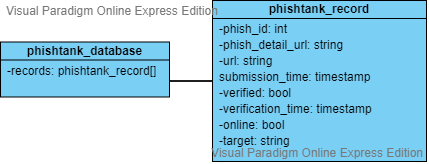
\includegraphics[width=0.5\textwidth]{images/phishtank_db.png}
\end{figure}

Columns are documented in the appendix \ref{appendix:phishtank_record}. 

Phishtank only provides the current state of its database, but we are also interested in the information of how long was website accessible. We will build our database alongside with this information in the following matter:
\begin{enumerate}
    \item Request a current state from Phishtank service
    \item If in our database are records with column \texttt{online=true} while they are not present in requested records, set them to \texttt{online=false} and create a new column \texttt{end\_time} with a current timestamp.
    \item Insert all records, which \texttt{phish\_id} isn't present in our database, into the database
\end{enumerate}

We had implemented this into JavaScript command-line utility, which will be periodically executed to update our database table \texttt{Phishtank}. Program with instructions is attached in the sources (\ref{appendix:phishurl_fetcher}).
%%%%%%%%%%%%%%%%%%%%

\subsection{URL anomalies detection}
\subsection{Behaviorial}
% TODO: whois, dns resolving, IP, /robots.txt...

% \subsection{And so on, this will be updated on the fly}

% \section{?Combining it together to a backend/proxy/module?}
% TODO: combine it and create configuration a production ready application from the modules. ?Probably use some machine learning to teach modules, what are best values for their detection approach, so I dont have to test it manually.? Write about 

% https://github.com/astaruch/master-thesis-everything/tree/master/code/phishing-app . 

% How to setup app.

% \section{?Frontend?}
% TODO: MAYBE IF THERE WILL BE TIME. Do a simple frontend for network administrator, so he can manually change behaviour of the app; e.g. add more values to some tests - enter google api key, refresh phishtank db, add new DNSBL and so on.

\chapter{Testing}

\section{Deployment}
% TODO: ideally create a Docker image for simple deployment on something like phishing-proxy.staruch.sk

\section{Integration into proxy}
% TODO: research possibility how to insert app into Kernun UTM/FW 

\section{Testing on real traffic}
% TODO: ideally, at least 2 weeks of testing - around march/april

\section{Results}
% TODO: prepare some graphs if this work is helpful or not, if speed of network is slower or unaffected, if customers are generally more happy, if newtork administrators can see some differences

\chapter{Summary}
% TODO: discuss what I did and if this thesis fulfills its goal



\shorthandon{-}


\printbibliography[heading=bibintoc] %% Print the bibliography.

\appendix
\chapter{Documentation}

\section{Phishtank record}
\label{appendix:phishtank_record}

% \begin{table}[]
\begin{tabularx}{\linewidth}{ r X }
\toprule
\textbf{phish\_id} & The ID number by which Phishtank refers to a phish submission. All data in PhishTank is tied to this ID. This will always be a positive integer. \\
\textbf{phish\_detail\_url} & PhishTank detail url for the phish, where you can view data about the phish, including a screenshot and the community votes. \\ \textbf{url} & The phish URL. This is always a string, and in the XML feeds may be a CDATA block. \\
\textbf{submission\_time} & The date and time at which this phish was reported to Phishtank. This is an ISO 8601 formatted date. \\
\textbf{verified} & Whether or not this phish has been verified by our community. In these data files, this will always be the string 'yes' since we only supply verified phishes in these files. \\
\textbf{verification\_time} & The date and time at which the phish was verified as valid by our community. This is an ISO 8601 formatted date. \\
\textbf{online} & Whether or not the phish is online and operational. In these data files, this will always be the string 'yes' since we only supply online phishes in these files. \\
\textbf{target} & The name of the company or brand the phish is impersonating, if it's known. \\ \bottomrule
\end{tabularx}
% \end{table}

\section{Phishurl fetcher}
\label{appendix:phishurl_fetcher}

\dirtree{%
.1 phishurl-fetcher. 
.2 README.md.
.2 docker-compose.yaml.
.2 ormconfig.json.
.2 package-lock.json.
.2  package.json.
.2  src.
.3     config.
.4     index.js.
.3     database.
.4     entity.
.5     LastUpdated.js.
.5     Phishtank.js.
.4     index.js.
.4     migration
.5     1555874663933-CreatePhishtank.js.
.5     1555897004589-CreateLastUpdated.js.
.4     model.
.5     LastUpdated.js.
.5     Phishtank.js.
.2     index.js.
.2     operations.
.3     last-updated.js.
.3     phishtank.js.
.2     utils.
.3     logger.js.
.3     utils.js.
}


\end{document}
